\documentclass[resume]{subfiles}



\begin{document}
\section{Buildroot}
\subsection{Répertoires}
\begin{figure}[H]
\centering
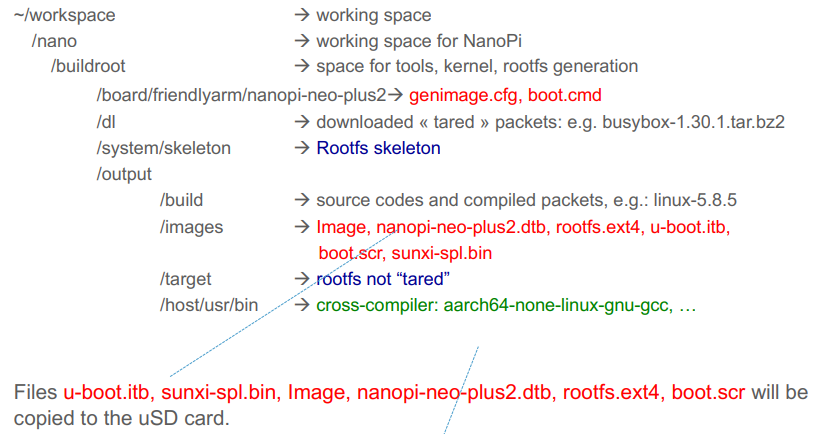
\includegraphics[width=0.9\columnwidth]{img_1.png}
\end{figure}
Ce qui est manquant dans le dossier output sera recompilé lorsque la commande \verb!make! est lancée (ou alors en faisant la commande\\
\verb!make <package>-rebuild!.\\
Le dossier \verb!rootfs_overlay! permet d'ajouter des fichiers au \verb!rootfs!\\
(\verb!/workspace/nano/buildrootboard/!\\
\verb!friendlyarm/nanopi-neo-plus2/rootfs_overlay!)
\subsection{Compilation}
Dans le répertoire \verb!buildroot!, effectuer la commande \verb!make menuconfig! puis \verb!make!. \verb!make clean! pour effacer tous les fichiers compilés.\\
La configuration permet notamment de 
\begin{enumerate}
\item Modifier le rootfs
\end{enumerate}
\subsection{Carte SD}
\begin{figure}[H]
\centering
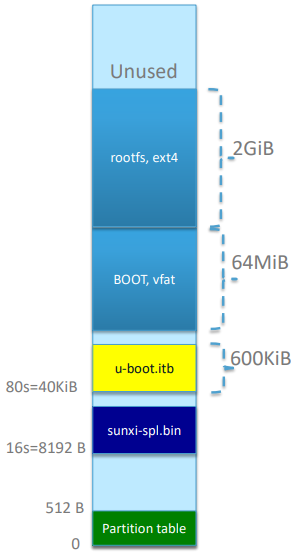
\includegraphics[height=\columnwidth,angle=90]{img_2.png}\\
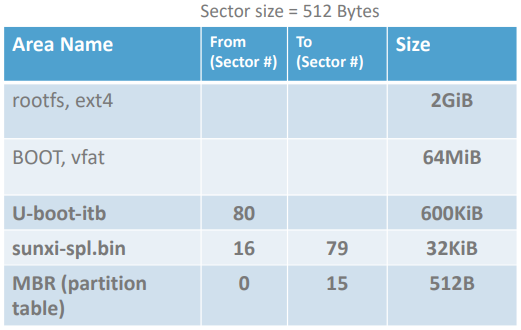
\includegraphics[width=0.5\columnwidth]{img_3.png}
\end{figure}
\begin{center}
\verb!genimage.cfg!$\longrightarrow$\verb!genimage!$\longrightarrow$\verb!sdcard.img!$\longrightarrow$\verb!dd!$\longrightarrow$ carte SD
\end{center}
Les fichiers pour l'initialisation sont\\
\begin{table}[H]
\begin{tabular}{ll}
\verb!rootfs.ext! & Root file system\\
\verb!Image! & Noyau Linux\\
\verb!nanopo-neo-plus2.dtb! & Flattened device tree\\
\verb!boot.scr! & Commandes boot compilées utilisées par u-boot\\
\verb!boot.vfat! & Partition boot\\
\verb!u-boot.itb! & Boot loader\\
\verb!sunxi-spl.bin! & Secondary Program Loader
\end{tabular}
\end{table}
\verb!boot.vfat! contient \verb!Image!, \verb!nanopi-neo-plus2.dtb! et \verb!boot.scr!. \verb!boot.vfat! (ou \verb!boot.ext4!) permet de créer \verb!BOOT! sur la carte SD
\subsubsection{rootfs}
Contient \verb!/bin!, \verb!/sbin!, \verb!/root!, \verb!/etc!, etc...
\subsubsection{boot.scr}
Le fichier \verb!boot.scr! est utilisé par u-boot pour charger le kernel Linux. Il est créé avec la commande \verb!mkimage!
\subsubsection{boot.cmd}
\verb!boot.cmd! contient des informations de démarrage, notamment les emplacements des différents l'emplacement de \verb!nanopi-neo-plus2.dtb!, du kernel et (si présent) de l'initramfs

\subsection{Séquence de démarrage (6 phases)}
\begin{enumerate}
\item Lorsque le $\mu$P est mis sous tension, le code stocké dans son BROM va charger dans ses 32KiB de SRAM interne le firmware \verb!sunxi-spl! stocké dans le secteur no 16 de la carte SD / eMMC et l’exécuter. 
\item Le firmware \verb!sunxi-spl! (Secondary Program Loader) initialise les couches basses du $\mu$P, puis charge l'U-Boot dans la RAM du $\mu$P avant de le lancer.
\item L'U-Boot va effectuer les initialisations hardware nécessaires (horloges, contrôleurs, …) avant de charger l’image non compressées du noyau Linux dans la RAM, le fichier \verb!Image!, ainsi que le fichier de configuration FDT (flattened device tree).
\item L'U-Boot lancera le noyau Linux en lui passant les arguments de boot (bootargs)
\item Le noyau Linux procédera à son initialisation sur la base des bootargs et des éléments de configuration contenus dans le fichier FDT (sun50i-h5-nanopi-neo plus2.dtb).
\item Le noyau Linux attachera les systèmes de fichiers (rootfs, tmpfs, usrfs, …) et poursuivra son exécution.
\end{enumerate}

\begin{figure}[H]
\centering
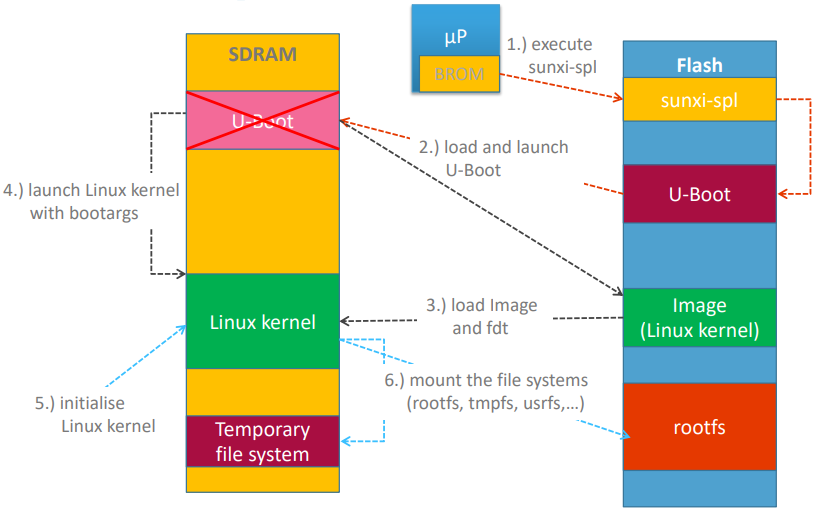
\includegraphics[width=\columnwidth]{img_4.png}
\end{figure}



\end{document}